\documentclass[12pt,a4paper]{article}
\usepackage[utf8]{inputenc}
\usepackage[swedish,shorthands=off]{babel}
\usepackage[widespace]{fourier}
\usepackage{setspace}
\usepackage[margin=2.5cm]{geometry}
\usepackage{csquotes}
\usepackage{graphicx}

% Blockcitat
\usepackage{relsize,etoolbox}
\AtBeginEnvironment{quote}{\smaller}

% Fotnoter
\usepackage[hang,flushmargin]{footmisc}
\interfootnotelinepenalty=10000

% Tabeller
\usepackage{booktabs}
\usepackage{siunitx}
\usepackage[singlelinecheck=false,labelfont=bf]{caption}
\makeatletter
\def\new@fontshape{}
\makeatother

% Diagram
\usepackage{pgfplots}
\pgfplotsset{compat=1.18}

% Innehållsförteckning
\addto\captionsswedish{\renewcommand{\contentsname}{Innehållsförteckning}}
\addto\captionsswedish{\renewcommand{\listtablename}{Tabellförteckning}}
\addto\captionsswedish{\renewcommand{\listfigurename}{Figurförteckning}}

% Undvik enkelrader i den mån det är möjligt
\widowpenalty=10000
\clubpenalty=10000

% Creative Commons-licens
\usepackage{ccicons}
\usepackage[type={CC},modifier={by-sa},version={4.0},]{doclicense}

% Litteraturförteckning
\usepackage[style=apa,backend=biber]{biblatex}
\addbibresource{Kandidatuppsats.bib}

% Glossering
\usepackage{gb4e}
\let\eachwordone=\it

% hyperref
\usepackage{hyperxmp}
\usepackage[hidelinks,linktoc=all]{hyperref}




% Uppsatsen börjar här %%%%%%%%%%%%%%%%%%%%%%%%%%%%%%%%%%%%%%%%%%%%%%%%%%%%%%%%%%%%%%%%%%%%%%%%%%%%%
%%%%%%%%%%%%%%%%%%%%%%%%%%%%%%%%%%%%%%%%%%%%%%%%%%%%%%%%%%%%%%%%%%%%%%%%%%%%%%%%%%%%%%%%%%%%%%%%%%%%
\begin{document}
% Romersk sidnumrering
\clearpage
\pagenumbering{roman}

% Metadata som används av hyperref
\title{Rörande bruket av mentala verb i japanska}
\author{Ingemar Berg}
\date{}

\hypersetup{keeppdfinfo,pdftitle={Rörande bruket av mentala verb i japanska},pdfauthor={Ingemar Berg}}




% Titelsida %%%%%%%%%%%%%%%%%%%%%%%%%%%%%%%%%%%%%%%%%%%%%%%%%%%%%%%%%%%%%%%%%%%%%%%%%%%%%%%%%%%%%%%%
%%%%%%%%%%%%%%%%%%%%%%%%%%%%%%%%%%%%%%%%%%%%%%%%%%%%%%%%%%%%%%%%%%%%%%%%%%%%%%%%%%%%%%%%%%%%%%%%%%%%
\hypersetup{pageanchor=false}

\begin{titlepage}
\noindent
\begin{minipage}[t]{6cm}
LUNDS UNIVERSITET \\
Språk- och litteraturcentrum
\end{minipage}
\hfill
\begin{minipage}[t]{6cm}
EXAMENSARBETE \\
Japanska: Kandidatkurs (JAPK12) \\
Vårterminen 2022
\end{minipage}

\begin{center}
\begin{LARGE}
\vskip 10em
\noindent
\textbf{Rörande bruket av mentala verb i japanska}
\end{LARGE}
\begin{Large}
\vskip 1em
\noindent
Ingemar Berg
\end{Large}
\end{center}

\vfill
\hfill
\noindent
\begin{minipage}[t]{6cm}
Handledare: Shinichiro Ishihara \\
Språk- och litteraturcentrum
\end{minipage}
\end{titlepage}




% Sammandrag %%%%%%%%%%%%%%%%%%%%%%%%%%%%%%%%%%%%%%%%%%%%%%%%%%%%%%%%%%%%%%%%%%%%%%%%%%%%%%%%%%%%%%%
%%%%%%%%%%%%%%%%%%%%%%%%%%%%%%%%%%%%%%%%%%%%%%%%%%%%%%%%%%%%%%%%%%%%%%%%%%%%%%%%%%%%%%%%%%%%%%%%%%%%
\hypersetup{pageanchor=true}

% 1,5 gånger radavstånd
\setstretch{1.5}

\newpage
\section*{Sammandrag}
I den här kandidatuppsatsen undersöks bruket av mentala verb bland L2-talare av japanska. Teoridelen behandlar den betydelse som evidentiella markörer och Kamios teori om informationsterritorium har för ämnet. Därefter redogörs för den kvantitativa studie som har utförts i form av en korpusundersökning. Den genomförda studien har hämtat sina data från en inlärarkorpus och försökt identifiera av vilka talare och i vilka sammanhang språkfel relaterade till mentala verb vanligen görs. Tre typer av språkfel har kunnat beläggas: hyperkorrektion, övergeneralisering samt transfer, oönskad påverkan från ett annat språk. Det har också funnits statistiskt säkerställda resultat som visat att mindre komplexa texter innehöll fler språkfel relaterade till ämnet än vad som hade kunnat förväntas av en jämn fördelning.

\bigskip
\noindent
\textbf{Nyckelord:} mentala verb, informationsterritorium, andraspråksinlärning, japanska

% Creative Commons-licens (CC-BY-SA 4.0)
% https://creativecommons.org/licenses/by-sa/4.0/deed.sv
\vfill
\doclicenseThis




% Författarens tack %%%%%%%%%%%%%%%%%%%%%%%%%%%%%%%%%%%%%%%%%%%%%%%%%%%%%%%%%%%%%%%%%%%%%%%%%%%%%%%%
%%%%%%%%%%%%%%%%%%%%%%%%%%%%%%%%%%%%%%%%%%%%%%%%%%%%%%%%%%%%%%%%%%%%%%%%%%%%%%%%%%%%%%%%%%%%%%%%%%%%
\newpage
\section*{Författarens tack}
Det skulle inte ha varit möjligt att skriva den här uppsatsen utan den handledning, den uppmuntran och de kloka råd som jag ständigt har fått av min handledare Shinichiro Ishihara. Jag är djupt tacksam för att du har delat med dig av din kunskap och tid så generöst. Tack också till Hannes Jansson-Möller som har varit ett stöd under hela skrivprocessen. Dina insikter i lateralt tänkande visade sig vara ovärderliga. Simon Lundahl och William Rylander har båda bidragit med kloka synpunkter, vilket jag är tacksam för. Till sist vill jag tacka Josefin Öhr som oavbrutet har uppmuntrat mig att fortsätta mina studier i japanska. Du fick mig att förstå allt och ingenting. Alla fel som återstår är mina egna.




% Innehållsförteckning %%%%%%%%%%%%%%%%%%%%%%%%%%%%%%%%%%%%%%%%%%%%%%%%%%%%%%%%%%%%%%%%%%%%%%%%%%%%%
%%%%%%%%%%%%%%%%%%%%%%%%%%%%%%%%%%%%%%%%%%%%%%%%%%%%%%%%%%%%%%%%%%%%%%%%%%%%%%%%%%%%%%%%%%%%%%%%%%%%
\clearpage

% Normalt radavstånd
\setstretch{1}

% Innehållsförteckning
\tableofcontents




% Tabell- och figurförteckning %%%%%%%%%%%%%%%%%%%%%%%%%%%%%%%%%%%%%%%%%%%%%%%%%%%%%%%%%%%%%%%%%%%%%
%%%%%%%%%%%%%%%%%%%%%%%%%%%%%%%%%%%%%%%%%%%%%%%%%%%%%%%%%%%%%%%%%%%%%%%%%%%%%%%%%%%%%%%%%%%%%%%%%%%%
\newpage

% Tabellförteckning
\listoftables

% Figurförteckning
\listoffigures




% Konventioner och förkortningar %%%%%%%%%%%%%%%%%%%%%%%%%%%%%%%%%%%%%%%%%%%%%%%%%%%%%%%%%%%%%%%%%%%
%%%%%%%%%%%%%%%%%%%%%%%%%%%%%%%%%%%%%%%%%%%%%%%%%%%%%%%%%%%%%%%%%%%%%%%%%%%%%%%%%%%%%%%%%%%%%%%%%%%%
% 1,5 gånger radavstånd
\setstretch{1.5}

\newpage
\section*{Konventioner och förkortningar}

% Konventioner och förkortningar
% Glossering
\subsection*{Glossering}
Leipzigreglerna för glossering (eng. \emph{Leipzig Glossing Rules}) används genomgående i uppsatsen. När glossering har saknats till exempelmeningar så har det utförts av mig i efterhand. En lista över de förkortningar som förekommer följer nedan \autocite{comrie2008}.

% Konventioner och förkortningar
% Transkribering
\subsection*{Transkribering}
En modifierad variant av Hepburn-systemet används för att transkribera japanska till det latinska alfabetet. Makroner används för att markera lång vokal, förutom långt \emph{e}, vilket i stället skrivs som \emph{ei}. Det innebär att jag till exempel skriver \emph{watashi} och inte \emph{watasi} 'jag', \emph{t\=omeiningen} och inte \emph{toumeiningen} 'osynlig person' och så vidare. Ord av japanskt ursprung som ingår i det svenska lexikonet av hävd använder dock den svenska stavningen, vilket exempelvis innebär att den japanska huvudstaden skrivs som \emph{Tokyo} och inte \emph{T\=oky\=o}. Alla översättningar är mina om inget annat anges.

% Konventioner och förkortningar
% Typografiska konventioner
\subsection*{Typografiska konventioner}
Kursiv text används för att markera utländska ord. Översättningar av såväl dessa som exempelmeningar till svenska omges av enkla citattecken. I övrigt används dubbla citattecken, till exempel för att ange direkta citat. När blockcitat förekommer markeras dessa i form av indrag och något mindre teckenstorlek.

% Konventioner och förkortningar
% Lista över förkortningar
\subsection*{Lista över förkortningar}
\begin{small}
\begin{tabular}{l p{3cm} l l}
\textsc{acc}  & ackusativ        & \textsc{neg}  & negation   \\
\textsc{comp} & komplementerare  & \textsc{nom}  & nominativ  \\
\textsc{cop}  & kopula           & \textsc{npst} & icke-dåtid \\
\textsc{dat}  & dativ            & \textsc{pass} & passiv     \\
\textsc{evid} & evidentialis     & \textsc{pol}  & artig stil \\
\textsc{foc}  & fokus            & \textsc{pst}  & dåtid      \\
\textsc{gen}  & genitiv          & \textsc{q}    & fråga      \\
\textsc{ger}  & gerundium        & \textsc{quot} & kvotativ   \\
\textsc{hon}  & respektfullt tal & \textsc{top}  & topik      \\
\end{tabular}
\end{small}




% Inledning %%%%%%%%%%%%%%%%%%%%%%%%%%%%%%%%%%%%%%%%%%%%%%%%%%%%%%%%%%%%%%%%%%%%%%%%%%%%%%%%%%%%%%%%
%%%%%%%%%%%%%%%%%%%%%%%%%%%%%%%%%%%%%%%%%%%%%%%%%%%%%%%%%%%%%%%%%%%%%%%%%%%%%%%%%%%%%%%%%%%%%%%%%%%%
% Normal sidnumrering
\clearpage
\pagenumbering{arabic}

\newpage
\section{Inledning}
\label{ch:Inledning}

% Inledning
% Ämnesval
\subsection{Ämnesval}
\label{sec:Inledning: Ämnesval}
Nybörjarstudenten av japanska har en avsevärd mängd material att sätta sig in i. De tre skrivsystemen \emph{hiragana}, \emph{katakana} och \emph{kanji} utgör tillsammans med ett lexikon och en grammatik utan tydliga kopplingar till västerländska språk kanske de mest uppenbara utmaningarna. Om inte förr så kommer de kulturella normernas påverkan på språket att utkristallisera sig någon gång mellan slutet av den första och början av den andra terminens studier. På goda grunder kan det antas att \emph{keigo}, det artighetsspråk som präglar hela den japanska kulturen, kommer att vara den mest påfallande kontakten med den aspekten av det japanska språket. Något som däremot verkar ges betydligt mindre utrymme är vad talaren av japanska kan påstå sig veta om sina medmänniskors känslor och upplevelser.\footnote{I nybörjarboken \emph{GENKI: An Integrated Course in Elementary Japanese I}, flitigt använd som kurslitteratur vid svenska universitets och högskolors nybörjarkurser i japanska, ägnas det några rader i kapitel 11, precis i slutet av den första terminens studier. Det hela utvecklas sedan en aning i kapitel 14 i fortsättningsboken \emph{GENKI: An Integrated Course in Elementary Japanese II} \autocite{banno2020a,banno2020b}.} En användare på \emph{Japanese Language Stack Exchange}, en webbplats där språkfrågor kan diskuteras, ger följande beskrivning:

\blockquote[{\cite{schaab2011}}]{Det japanska språket har en märklig oskriven regel som i huvudsak säger att man inte kan anta att man känner till de innersta detaljerna i en tredje persons mentala tillstånd. [...] Till och med om din son har tjatat på dig i sex veckor i rad att du ska ge honom en av de där splitternya \mbox{DS-grunkorna}\footnote{Här anspelar författaren på Nintendo DS, en vid textens författande mycket populär spelkonsol.} (eftersom alla hans vänner har en, till och med Kentarō, vars föräldrar aldrig köper något till honom) och fast att du är hundra procent säker på att han vill ha en [Nintendo] DS så kan du inte säga det rakt ut.}

\noindent
Just det som användaren kallar för \emph{en märklig oskriven regel} kommer att stå i centrum för min uppsats. Mer formellt benämns denna typ av fenomen som beskriver mentala tillstånd av olika slag \emph{mentala verb}. Dessa förekommer i ett flertal språk och används i huvudsak för att uttrycka vad en person känner eller upplever. I en del västerländska språk, såsom svenska eller engelska, görs det ingen skillnad mellan när talaren och någon annan person gör detta. Det står i skarp kontrast till japanska, där det i flera fall finns starka restriktioner på användningen av mentala verb \autocite{hasegawa2005}. Med utgångspunkt i dessa restriktioner avser jag att undersöka om L2-talare av japanska behärskar detta språkbruk samt vilka eventuella språkfel som kan förekomma till följd av det.

% Inledning
% Uppsatsens disposition
\subsection{Uppsatsens disposition}
\label{sec:Inledning: Uppsatsens disposition}
Uppsatsen är indelad i sex kapitel, där denna inledning utgör det första av dessa. I det andra kapitlet ger jag en bakgrund till fenomenet mentala verb. En kortare översikt över evidentialitet och evidentiella markörer samt vanliga språkfel och den forskning som finns kring de misstag som L2-talare av japanska gör ingår också. Det tredje kapitlet behandlar den genomförda undersökningen. Här redogörs för uppsatsens syfte och frågeställningar. De metodval som har gjorts beskrivs och motiveras och det praktiska genomförandet av undersökningen redovisas också här. I det fjärde kapitlet presenterar jag sedan resultaten från min undersökning. Det femte kapitlet innehåller en diskussion kring och en analys av den genomförda undersökningen. Möjliga ämnen för framtida forskning berörs också kort. I det sjätte och sista kapitlet sammanfattar jag avslutningsvis de slutsatser som har kunnat dras utifrån undersökningens resultat.




% Bakgrund %%%%%%%%%%%%%%%%%%%%%%%%%%%%%%%%%%%%%%%%%%%%%%%%%%%%%%%%%%%%%%%%%%%%%%%%%%%%%%%%%%%%%%%%%
%%%%%%%%%%%%%%%%%%%%%%%%%%%%%%%%%%%%%%%%%%%%%%%%%%%%%%%%%%%%%%%%%%%%%%%%%%%%%%%%%%%%%%%%%%%%%%%%%%%%
\newpage
\section{Bakgrund}
\label{ch:Bakgrund}
I bakgrundskapitlet redogörs för den teori som är nödvändig för att kunna förklara bruket av mentala verb ur en språkinlärares perspektiv. Jag inleder med ett kortare avsnitt som behandlar evidentialitet och evidentiella markörer, vilket är av vikt för att förstå de restriktioner som finns på användningen av mentala verb. Därefter följer en diskussion kring just dessa, där exempel på såväl acceptabelt som oacceptabelt språkbruk ges. Några vanliga typer av språkfel presenteras sedan och avslutningsvis sammanfattas den tidigare forskning som finns kring de språkfel som L2-talare av japanska gör.

% Bakgrund
% Evidentiella markörer
\subsection{Evidentiella markörer}
\label{sec:Bakgrund: Evidentiella markörer}
Evidentialitet, det vill säga hur och på vilket sätt talaren har tillgodogjort sig information om en inträffad händelse, spelar en central roll i det japanska språket. Evidentiella markörer av någon form är därför ofta nödvändiga för att kunna återge en annan människas tankar eller känslor på ett acceptabelt sätt. Det är således genom användandet av sådana markörer som talaren visar att denne inte har direkt tillgång till en annan människas inre liv, vilket i sin tur anknyter till det resonemang om oskrivna kulturella regler som har förts ovan. En avgörande fråga för att kunna fastställa om någon evidentiell markör behövs i ett visst sammanhang är talarens tillgång till information \autocite{kuno1973,shibatani1990}.

\textcite{kamio1994,kamio1995} hävdar att användandet av exempelvis satsfinala partiklar och evidentiella markörer är direkt beroende av just talarens tillgång till information. Han menar att varje talare har sitt eget informationsterritorium och att sättet som talaren och andra aktörer förhåller sig till det med nödvändighet behöver variera, för att ett samtal ska upplevas som naturligt. Det exemplifieras enligt följande:

\blockquote[{Fritt översatt från \cite[315]{hasegawa2015}}]{John, chefen för ett företag, och Tom, hans affärspartner, har ett möte på Johns kontor. [...] Johns sekreterare informerar honom om att han har ett [nytt] möte klockan tre. När klockan så närmar sig tre vore det naturligt för John att säga: \emph{Jag har ett [nytt] möte klockan tre}. Skulle däremot Tom säga: \emph{Du har ett möte klockan tre} så hade det sannolikt gett ett märkligt intryck. Trots att både John och Tom har tagit del av informationen anses den höra till Johns informationsterritorium, då den bara berör honom. [...] Tom behöver därför vara mer försiktig i sitt påstående och kan i stället exempelvis säga: \emph{Jag har förstått att du har ett nytt möte klockan tre}.}

\noindent
Det finns således en betydande skillnad mellan när talaren har kännedom om något som angår denne själv jämfört med när det berör en annan person. När kunskap om en händelse finns i talarens informationsterritorium, behöver det uttryckas utan hjälp av någon evidentiell markör. På motsvarande sätt behöver särskild hänsyn tas till mer indirekta formuleringar, när kunskapen i stället hör till en annan människas informationsterritorium. Vilken evidentiell markör som kan användas beror i sin tur på hur och på vilket sätt informationen har inhämtats \autocite{kamio1994,kamio1995,hasegawa2015,shibatani1990}.

Om talaren som i (\ref{ex:Makino1}) utgår från kunskap som denne har inhämtat genom att exempelvis läsa eller lyssna, bör i första hand den evidentiella markören \emph{rashii} användas. Vidare är \emph{s\=oda} ett passande val när påståendet i stället har sin grund i talarens visuella intryck, vilket visas i (\ref{ex:Makino2}). Avslutningsvis kan \emph{y\=oda} fungera som evidentiell markör när talaren likt i (\ref{ex:Makino3}) baserar sin utsaga på ett logiskt resonemang \autocite{makino1986}.

\begin{exe}
\ex
\begin{xlist}
\ex
\label{ex:Makino1}
\gll Kono hon wa takai rashi-i. \\
     denna bok \textsc{top} dyr \textsc{evid}-\textsc{npst} \\
\glt 'Den här boken verkar vara dyr (baserat på vad jag har läst eller hört).'
\ex
\label{ex:Makino2}
\gll Kono hon wa taka s\=o-da. \\
     denna bok \textsc{top} dyr \textsc{evid}-\textsc{cop}.\textsc{npst} \\
\glt 'Den här boken ser ut att vara dyr.'
\ex
\label{ex:Makino3}
\gll Kono hon wa takai y\=o-da. \\
     denna bok \textsc{top} dyr \textsc{evid}-\textsc{cop}.\textsc{npst} \\
\glt 'Den här boken verkar vara dyr (jämfört med vad andra böcker kostar).'
\flushright \autocite[551]{makino1986}
\end{xlist}
\end{exe}

\noindent
En annan vanligt förekommande evidentiell markör är suffixet \emph{garu}, att någon annan än talaren ger sken av att vilja eller uppleva någonting. Det behöver ofta användas när någon annan persons inre liv berörs och spelar således en central roll för bruket av mentala verb \autocite{makino1986}.

% Bakgrund
% Mentala verb
\subsection{Mentala verb}
\label{sec:mentalaverb}
I det här avsnittet kommer bruket av mentala verb att systematiskt presenteras för såväl första som andra och tredje person. Både acceptabel och oacceptabel användning illustreras med ett flertal exempel ur litteraturen. Avslutningsvis berörs också när och i vilka typer av satser som bruket av mentala verb tillåts.

% Bakgrund
% Mentala verb
% Användning av mentala verb i första person
\subsubsection{Användning av mentala verb i första person}
\label{subsec:Bakgrund: Mentala verb: Användning av mentala verb i första person}
Det sätt på vilket mentala verb används i japanska är flitigt diskuterat i litteraturen, även om förklaringarna som ges kan skilja sig något åt. \textcite{hasegawa2015} menar exempelvis att det inte finns någon explicit grammatiskt förklaring till varför de ofta inte kan användas i andra eller tredje person. I stället handlar det om en kulturell insikt i att det är omöjligt att förstå vad som sker i en annan människas inre liv. Vid dessa tillfällen behöver således någon evidentiell markör användas, vilket visas nedan:

\begin{exe}
\ex
\begin{xlist}
\ex
\label{ex:Hasegawa1a}
\gll Watashi wa samu-i. \\
     jag \textsc{top} frusen-\textsc{npst} \\
\glt 'Jag är frusen.'
\ex
\label{ex:Hasegawa1b}
\gll Arisu wa samu-gat-te i-ru. \\
     {} \textsc{top} frusen-\textsc{evid}-\textsc{ger} vara-\textsc{npst} \\
\glt 'Alice ger sken av att vara frusen.'
\hfill \autocite[313]{hasegawa2015}
\end{xlist}
\end{exe}

\begin{exe}
\ex
\begin{xlist}
\ex
\label{ex:Hasegawa2a}
\gll Watashi wa k\=oh\={\i} ga hoshi-i. \\
     jag \textsc{top} kaffe \textsc{nom} vill-\textsc{npst} \\
\glt 'Jag vill ha (lite) kaffe.'
\ex
\label{ex:Hasegawa2b}
\gll Arisu wa k\=oh\={\i} o hoshi-gat-te i-ru. \\
     {} \textsc{top} kaffe \textsc{acc} vill-\textsc{evid}-\textsc{ger} vara-\textsc{npst} \\
\glt 'Alice ger sken av att vilja ha kaffe.'
\hfill \autocite[313--314]{hasegawa2015}
\end{xlist}
\end{exe}

\noindent
Såväl (\ref{ex:Hasegawa1a}) som (\ref{ex:Hasegawa2a}) berör olika sorters mentala tillstånd, nämligen upplevelsen av att vara frusen respektive av att vilja ha någonting. Här begränsas inte talaren i att uttrycka hur denne upplever situationen, då båda dessa exempel utgörs av påståendesatser i första person. I (\ref{ex:Hasegawa1b}) och (\ref{ex:Hasegawa2b}) tydliggörs hur motsvarande situation beskriven i tredje person i stället kräver att en evidentiell markör används \autocite{hasegawa2015,hasegawa2005}.

På motsvarande vis finns det, åtminstone till viss del, restriktioner på bruket av \emph{garu} i första person. \textcite{kuroda1973} menar att (\ref{ex:Kuroda1}) ger ett onaturligt intryck, även om han inte hävdar att meningen är ogrammatisk. En möjlig förklaring som ges är att bruket av \emph{garu} i första person implicerar att talaren både observerar ett känslointryck och samtidigt själv upplever det, vilket kan uppfattas som motsägelsefullt.

\begin{exe}
\ex[?]{
\label{ex:Kuroda1}
\gll Watashi wa atsu-gat-te i-ru. \\
     jag \textsc{top} varm-\textsc{evid}-\textsc{ger} vara-\textsc{npst} \\
\glt 'Jag ger sken av att vara varm.'
\hfill \autocite[anpassat från][378]{kuroda1973}}
\end{exe}

Både \textcite{kuno1973} och \textcite{kuroda1973} påpekar att det finns tillfällen när mentala verb inte kan användas i första person. Eftersom talarens mentala tillstånd är uppenbart enbart för denne själv och inte någon annan människa, tillåts följaktligen inte heller frågesatser i första person. I (\ref{ex:Kuroda2a}) tydliggörs denna oacceptabla användning. Däremot är (\ref{ex:Kuroda2b}) acceptabel, då restriktionen i stället saknas på frågesatser i andra person.

\begin{exe}
\ex
\begin{xlist}
\ex[*]{
\label{ex:Kuroda2a}
\gll Watashi wa atsui desu ka? \\
     jag \textsc{top} varm \textsc{cop}.\textsc{pol}.\textsc{npst} \textsc{q} \\
\glt 'Är jag varm?'}
\ex[]{
\label{ex:Kuroda2b}
\gll Anata wa atsui desu ka? \\
     du \textsc{top} varm \textsc{cop}.\textsc{pol}.\textsc{npst} \textsc{q} \\
\glt 'Är du varm?'
\hfill \autocite[anpassat från][378]{kuroda1973}}
\end{xlist}
\end{exe}

% Bakgrund
% Mentala verb
% Användning av mentala verb i andra person
\subsubsection{Användning av mentala verb i andra person}
\label{subsec:Bakgrund: Mentala verb: Användning av mentala verb i andra person}
\textcite{pettersson1995} antar i huvudsak en liknande ståndpunkt som \textcite{hasegawa2015}. Han instämmer i att de tillfällen när mentala verb kan användas annat än i första person är begränsade; det är just svårigheten i att få insikt i en annan människas inre liv som förhindrar detta. En skillnad är dock att Pettersson också berör bruket av mentala verb i andra person. Det kulturellt godtagbara fallet med frågesatser rörande en interlokutörs känslor eller upplevelser visade i (\ref{ex:Kuroda2b}) ovan. Några ytterligare exempel från litteraturen följer nedan:

\begin{exe}
\ex
\label{ex:Kuno1}
\gll Kono hon ga yomi-ta-i? \\
     denna bok \textsc{nom} läsa-vill-\textsc{npst} \\
\glt 'Vill du läsa den här boken?'
\hfill \autocite[anpassat från][336]{kuno1973}
\end{exe}

\begin{exe}
\ex
\label{ex:Makino4}
\gll Ky\=o wa nani ga tabe-tai desu ka? \\
     {i dag} \textsc{top} vad \textsc{nom} äta-vill \textsc{cop}.\textsc{pol}.\textsc{npst} \textsc{q} \\
\glt 'Vad vill du äta i dag?'
\hfill \autocite[anpassat från][443]{makino1986}
\end{exe}

\begin{exe}
\ex
\label{ex:Makino5}
\gll Anata wa ima nani ga hoshii desu ka? \\
     du \textsc{top} nu vad \textsc{nom} vill \textsc{cop}.\textsc{pol}.\textsc{npst} \textsc{q} \\
\glt 'Vad vill du ha nu?'
\hfill \autocite[anpassat från][144]{makino1986}
\end{exe}

\noindent
I såväl (\ref{ex:Kuno1}) som (\ref{ex:Makino4}) och (\ref{ex:Makino5}) ges ytterligare belägg för hur bruket av mentala verb i frågesatser i andra person är acceptabelt. Mer indirekta formuleringar kan dock också förekomma beroende på situation och artighetsnivå. Graden av artighet, vilken i sig är en direkt följd av relationen mellan talaren och dennes interlokutör, påstås vara starkt kopplad till huruvida en direkt fråga är lämplig eller ej. Ju närmare relation, desto mer direkt är det möjligt att fråga om exempelvis önskemål \autocite{pettersson1995}.\footnote{Samtliga översättningar av exempelmeningar hämtade ur \textcite{pettersson1995} är hans och inte mina.}

\begin{exe}
\ex
\label{ex:Pettersson1}
\gll {Nani ka} hoshii mono a-ru? \\
     någonting vill föremål vara-\textsc{npst} \\
\glt 'Är det någonting du vill ha?'
\hfill \autocite[anpassat från][87]{pettersson1995}
\end{exe}

\begin{exe}
\ex
\begin{xlist}
\ex[*]{
\label{ex:Pettersson2a}
\gll {Go-issho ni} iki-tai desu ka? \\
     \textsc{hon}-tillsammans gå-vill \textsc{cop}.\textsc{pol}.\textsc{npst} \textsc{q} \\
\glt 'Vill Ni gå med?'}
\ex[]{
\label{ex:Pettersson2b}
\gll {Go-issho ni} ikaga desu ka? \\
     \textsc{hon}-tillsammans hur.\textsc{pol} \textsc{cop}.\textsc{pol}.\textsc{npst} \textsc{q} \\
\glt 'Vill Ni gå med?'}
\ex[]{
\label{ex:Pettersson2c}
\gll {Go-issho ni} ika-re-masen ka? \\
     \textsc{hon}-tillsammans gå-\textsc{pass}-\textsc{neg}.\textsc{pol}.\textsc{npst} \textsc{q} \\
\glt 'Vill Ni gå med?'
\hfill \autocite[anpassat från][86]{pettersson1995}}
\end{xlist}
\end{exe}

Bruket av mentala verb i frågesatser tillåts i familjära sammanhang, där artighetsnivån är låg likt i (\ref{ex:Pettersson1}). \textcite{pettersson1995} menar vidare att (\ref{ex:Pettersson2a}) är oacceptabel, då det vore alltför personligt att ställa en direkt fråga i ett formellt sammanhang. I stället bör talaren uttrycka sig mer indirekt i den sortens situationer. Av (\ref{ex:Pettersson2b}) och (\ref{ex:Pettersson2c}) framgår hur en sådan fråga skulle kunna formuleras på ett kulturellt godtagbart sätt. Båda dessa exempel innehåller olika former av \emph{sonkeigo} 'respektfullt tal', vilket vore mer lämpligt i denna kontext.

Det finns en samstämmighet i litteraturen om att mentala verb kan användas i frågesatser i andra person. Varken \textcite{kuno1973} eller \textcite{makino1986} nämner däremot sambandet mellan direkthet och artighetsnivå, utan konstaterar i huvudsak att det vore alltför förenklat att påstå att mentala verb enbart kan användas i första person. Det påståendet utvecklas vidare i följande avsnitt, där bruket av mentala verb i tredje person behandlas.

% Bakgrund
% Mentala verb
% Användning av mentala verb i tredje person
\subsubsection{Användning av mentala verb i tredje person}
\label{subsec:Bakgrund: Mentala verb: Användning av mentala verb i tredje person}
Det har tidigare redogjorts för hur någon evidentiell markör behöver användas, när en tredje persons känslor eller upplevelser diskuteras. I litteraturen finns det exempel på den betydelseförskjutning som kan uppstå om talaren inte tar hänsyn till det. Ett exempel på hur en menings innebörd kan förändras visas nedan:

\begin{exe}
\ex
\begin{xlist}
\ex
\label{ex:HasegawaHirose1a}
\gll Watashi wa kanashi-i. \\
     jag \textsc{top} ledsen-\textsc{npst} \\
\glt 'Jag är ledsen.'
\ex
\label{ex:HasegawaHirose1b}
\gll Haha wa kanashi-i. \\
     mor \textsc{top} ledsen-\textsc{npst} \\
\glt 'Min mor gör mig ledsen.' inte 'Min mor är ledsen.'\footnote{Det bör dock nämnas att alla modersmålstalare inte nödvändigtvis delar denna uppfattning. När jag diskuterade frågan med min handledare, har hans upplevelse av meningen varit just den betydelse som enligt \textcite{hasegawa2005} inte kunde förekomma (S. Ishihara, personlig kommunikation, 8 april 2022).}
\flushright \autocite[229]{hasegawa2005}
\end{xlist}
\end{exe}

\noindent
\textcite{hasegawa2005} hävdar att bruket av mentala verb i tredje person är så pass rigoröst att meningens innebörd med nödvändighet förändras. I  (\ref{ex:HasegawaHirose1a}) blir betydelsen den förväntade, \emph{jag är ledsen}. Innebörden av (\ref{ex:HasegawaHirose1b}) blir däremot en annan. Den betydelse som torde ha förväntats, \emph{min mor är ledsen}, kan inte uttryckas utan en evidentiell markör. I litteraturen finns det dock också exempel på när dessa restriktioner kan bortfalla.

\begin{exe}
\ex
\label{ex:Makino6}
\gll M\=orisu wa ii sutereo ga hoshi-katta. \\
     {} \textsc{top} bra stereo \textsc{nom} vill-\textsc{pst} \\
\glt 'Maurice ville ha en bra stereo.'
\hfill \autocite[anpassat från][145]{makino1986}
\end{exe}

\noindent
Inledningsvis är det acceptabelt att använda mentala verb i dåtid, vilket kan ses i (\ref{ex:Makino6}). Det har tidigare nämnts att det är talarens brist på information om den inträffade händelsen som medför krav på en evidentiell markör. I detta fall anses denne dock ha haft fullgod möjlighet att kunna tillgodogöra sig informationen, vilket i sin tur ger att restriktionen inte längre kan komma i fråga \autocite{makino1986,shibatani1990}.

\begin{exe}
\ex
\label{ex:Makino7}
\gll Joi mo hoshii to it-te i-ru. \\
     {} \textsc{foc} vill \textsc{quot} säga-\textsc{ger} vara-\textsc{npst} \\
\glt 'Joy säger att hon också vill ha det.'
\hfill \autocite[anpassat från][145]{makino1986}
\end{exe}

\noindent
Vidare är det acceptabelt att återge vad en annan person själv har uttryckt rörande sina egna känslor eller upplevelser, vilket visas i (\ref{ex:Makino7}). I detta fall gör talaren ingen egen bedömning av personens upplevelser, utan redogör enbart för vad denne själv har sagt. Talaren saknar inte heller i det här fallet tillgång till information, vilket innebär att någon evidentiell markör inte behöver användas \autocite{makino1986,mcgloin1989}.

\begin{exe}
\ex
\label{ex:McGloin1}
\gll Tar\=o wa kuruma ga hoshii kara,  arubaito o shi-te i-ru. \\
     {} \textsc{top} bil \textsc{nom} vill eftersom arbete \textsc{acc} göra-\textsc{ger} vara-\textsc{npst} \\
\glt 'Tar\=o arbetar eftersom han vill ha en bil.'
\hfill \autocite[anpassat från][121]{mcgloin1989}
\end{exe}

\noindent
Avslutningsvis är det acceptabelt att använda mentala verb i bisatser likt (\ref{ex:McGloin1}). Det finns enligt \textcite{mcgloin1989} fall när detta bruk kan vara såväl acceptabelt som oacceptabelt. Det väsentliga är ur vilket perspektiv ett mentalt tillstånd beskrivs. När talaren, som i detta fall, gör det ur en tredje persons synvinkel är det acceptabelt.

Både \textcite{kamio1995} och \textcite{kuroda1973} redogör slutligen för hur valet av stil i en text kan påverka bruket av mentala verb. När ett allvetande berättarperspektiv används, vilket torde vara vanligast i skönlitteratur, så är författaren betydligt friare att uttala sig om känslor och upplevelser. Den skillnad som detta medför följer nedan:

\begin{exe}
\ex
\begin{xlist}
\ex
\label{ex:Kuroda3a}
\gll Yamadera no kane o kii-te, Mearii wa kanashi-katta. \\
     bergstempel \textsc{gen} klocka \textsc{acc} höra-\textsc{ger} {} \textsc{top} ledsen-\textsc{pst} \\
\glt 'Mary var ledsen när hon hörde bergstemplets klocka.'
\ex
\label{ex:Kuroda3b}
\gll Yamadera no kane o kii-te, Mearii wa kanashi-gat-ta. \\
     bergstempel \textsc{gen} klocka \textsc{acc} höra-\textsc{ger} {} \textsc{top} ledsen-\textsc{evid}-\textsc{pst} \\
\glt 'Mary var ledsen när hon hörde bergstemplets klocka.'
\flushright \autocite[anpassat från][384]{kuroda1973}
\end{xlist}
\end{exe}

\noindent
I (\ref{ex:Kuroda3a}) är texten skriven ur ett allvetande berättarperspektiv, vilket gör det möjligt för författaren att uttala sig om alla karaktärers inre liv utan några särskilda begränsningar. Väljer författaren i stället ett förstapersonsperspektiv så behöver denne på omvänt sätt ta hänsyn till hur den aktuella karaktären uppfattar sin omgivning. Det visas i (\ref{ex:Kuroda3b}) genom användningen av en evidentiell markör \autocite{kamio1995,kuroda1973}.

% Bakgrund
% Språkfel
\subsection{Språkfel}
\label{sec:Bakgrund: Språkfel}
I det här avsnittet kommer först några vanligt förekommande språkfel att presenteras. De har inte nödvändigtvis någon direkt koppling till just japanska, utan torde kunna motsvara de utmaningar som varje inlärare av ett främmande språk ställs inför. Därefter sammanfattas i korthet den tidigare forskning som finns kring de språkfel som L2-talare av japanska gör. Denna sammanfattning gör inget anspråk på att vara fullständig utan bör ses som en översikt över forskningsområdet.

% Bakgrund
% Språkfel
% Hyperkorrektion
\subsubsection{Hyperkorrektion}
\label{subsec:Bakgrund: Språkfel: Hyperkorrektion}
I \textcite[390]{språkriktighetsboken2011} beskrivs begreppet \emph{hyperkorrektion} enligt följande: "[Ett] språkbruk som är felaktigt och som har uppkommit genom språkbrukarens överdrivna ambition att uttrycka sig korrekt." Det är huvudsakligen när talaren försöker använda en grammatisk regel i en situation där den inte är tillämpbar, i stället för att följa sin språkkänsla, som detta fenomen kan uppstå \autocite{menner1937}.\footnote{Det får sägas ligga i sakens natur att hyperkorrektioner uppstår när talarens språkkänsla inte är tillräckligt väl utvecklad för att kunna avgöra vad som är grammatiskt och ej. Om den hade varit det, hade det inte heller funnits något behov av att luta sig mot en grammatisk regel från första början.} I svenskan skulle felaktig användning av \emph{de} och \emph{dem} i skrift kunna vara ett exempel på en hyperkorrektion, vilket visas i såväl (\ref{ex:Språkriktighetsboken1}) som (\ref{ex:Språkriktighetsboken2}). Det verkar finnas belägg för att också den som är osäker på hur de används korrekt föredrar \emph{de} och \emph{dem} i skrift trots att såväl subjekts- som objektsformen innefattas i \emph{dom} och därför borde vara ett säkrare val för en osäker talare \autocite{språkriktighetsboken2011}.

\begin{exe}
\ex[*]{\label{ex:Språkriktighetsboken1} Vad kostar dem?
\hfill \autocite[207]{språkriktighetsboken2011}}
\ex[*]{\label{ex:Språkriktighetsboken2} Dem här har vi till ett riktigt bra pris.\footnote{I det här exemplet fyller \emph{de} rollen som artikel och inte pronomen. Det är enbart när \emph{de} fungerar som pronomen som det kan ersättas av \emph{dom}. Det vore således felaktigt att göra den substitutionen här.}
\hfill \autocite[208]{språkriktighetsboken2011}}
\end{exe}

% Bakgrund
% Språkfel
% Övergeneralisering
\subsubsection{Övergeneralisering}
\label{subsec:Bakgrund: Språkfel: Övergeneralisering}
I senare forskning kring andraspråksinlärning verkar hyperkorrektioner snarare förstås med utgångspunkt i begreppet \emph{övergeneralisering}. \textcite[33]{viberg1987} ger följande förklaring: "Med övergeneralisering menas att en regel tillämpas för generellt." Han exemplifierar med både morfologiska och syntaktiska språkfel, där felaktig böjning av ett substantivs pluralform kan vara ett exempel på det tidigare. I (\ref{ex:Viberg1}) visas hur ett böjningsmönster tillämpas alltför generellt. I stället för att \emph{bror} böjs till \emph{bröder} blir i stället pluralformen felaktigt \emph{brorar}. Vidare kan ett exempel på ett syntaktiskt misstag ses i (\ref{ex:Viberg2}), där svenskans reflexiva pronomen \emph{sig}, vilket bara kan användas i tredje person, har fått en ogrammatisk användning \autocite{viberg1987}.

\begin{exe}
\ex
\begin{xlist}
\ex[*]{\label{ex:Viberg1} Hon besöker sina brorar varje helg.}
\ex[*]{\label{ex:Viberg2} Jag ska ta av sig jackan och hänga den på galgen.
\flushright \autocite[anpassat från][33-34]{viberg1987}}
\end{xlist}
\end{exe}

När en grammatisk regel lärs in av L2-talare finns det belägg för följande process: Från att först inte ha använts alls börjar den stegvis praktiseras. Vid det här stadiet faller sannolikt vissa av de restriktioner som finns på regelns tillämpning bort; dess användning övergeneraliseras. Språkkänslan utvecklas sedan successivt och regeln kan till sist tillämpas korrekt \autocite{viberg1987}.

% Bakgrund
% Språkfel
% Påverkan från andra språk
\subsubsection{Påverkan från andra språk}
\label{subsec:Bakgrund: Språkfel: Påverkan från andra språk}
Under språkinlärningsprocessen kan det förekomma att det nya språket påverkas av ett som talaren redan behärskar, antingen av talarens modersmål eller av något annat språk som denne har lärt sig. I forskningen kring andraspråksinlärning görs en åtskillnad mellan när det sker medvetet, så kallad \emph{kodväxling}, och när det inträffar omedvetet, vilket benämns \emph{transfer} \autocite{viberg1987}. Här ligger fokus på det senare begreppet. Följande text, skriven på svenska av en inlärare med engelska som modersmål, illustrerar olika typer av språkfel:

\blockquote[{\cite[50]{viberg1987}}]{Jag heter XX och jag kommer från Winter Park, Florida, USA. Nu, jag bor med en svenka familijen på Jakobsberg. Jag har varit på Sverige for sex veckor och med familjen for tre veckor. Jag har hitta det svenska är mycket svart att larare mig. Jag ska vara på Stockholm for bara ett år, sen kommer jag tillbaka USA. Jag ska sluta utbildningens dar, på universitetet av Florida. När forstare jag och pratar mer svenska, jag tror att jag ska tycker om Sverige betre. Men, jag har traffadat många, mycket snell svenka personar. [\emph{sic!}]\footnote{Texten innehåller alltför många fel för att det skulle vara praktiskt möjligt att markera varje enskilt sådant utan att inkräkta på läsbarheten. Då den används för att illustrera de språkfel som kan ske under en inlärningsprocess, vore det inte heller lämpligt att rätta dessa. Det är min förhoppning att denna kompromiss med en markering i slutet av citatet likväl ska vara godtagbar.}}

\noindent
\textcite{viberg1987} identifierar flera exempel på transfer. I meningen \emph{jag bor med en svenka familijen} ... hänför sig det felaktiga valet av preposition sannolikt till påverkan från talarens modersmål. Motsvarande mening på engelska skulle använda sig av \emph{with}. Samma typ av fel går också att se i \emph{universitetet av Florida}, där det engelska namnet på lärosätet, \emph{University of Florida}, torde ha påverkat den felaktiga översättningen till svenska. Det finns också exempel på övergeneralisering i form av de felaktiga konstruktionerna \emph{på Jakobsberg}, \emph{på Sverige} och \emph{på Stockholm}. Då \emph{på} är svenskans vanligaste rumspreposition, verkar det sannolikt att den grammatiska regeln för dess användning har övergeneraliserats. Det felaktiga valet av preposition torde inte bero på påverkan från talarens modersmål, eftersom motsvarande engelska konstruktion kräver att \emph{in} och inte \emph{on} används \autocite{viberg1987}.

% Bakgrund
% Språkfel
% Tidigare forskning
\subsubsection{Tidigare forskning}
\label{subsec:Bakgrund: Språkfel: Tidigare forskning}
\textcite{nishina2014} har i sin forskning analyserat språkfel i texter författade av L2-talare av japanska. Varje enskilt språkfel har inledningsvis betraktats med utgångspunkt i exempelvis meningsbyggnad, ordval eller fonologi. Därefter har det klassificerats utifrån vad som var ogrammatiskt, hur språkfelet yttrade sig samt vad som torde ha föranlett det. De huvudsakliga orsakerna som identifierades var följande:

\begin{enumerate}
\item Felaktigt val av stilnivå.
\item Likhet i betydelse, skrivtecken eller uttal.
\item Påverkan från modersmål.
\end{enumerate}

Knappt en tredjedel av felorsakerna visade sig ha sin grund i felaktigt val av stilnivå. Det fanns belägg för att en alltför ledig stil med inslag från nybörjarkursernas konversationslektioner påverkade det akademiska skrivandet negativt. Några exempel som gavs var förekomsten av den satsfinala partikeln \emph{ne}, vilken bland annat används för att söka bekräftelse av en utsaga, och valet av det informella verbet \emph{yaru} 'att göra' i en kontext, där den formella motsvarigheten \emph{suru} skulle ha varit mer i linje med textens förväntade stilnivå \autocite{nishina2014}.

Vidare fann \textcite{nishina2014} belägg för att en typ av fel kunde ha sin orsak i såväl likhet i uttal som skrivtecken. Det exemplifierades med att skriva \emph{y\=umei} 'berömd' när \emph{yume} 'dröm' var vad som avsågs. Här gavs det snarlika uttalet hos orden som förklaring till språkfelet. Den här sortens fel förekom främst bland de talare som saknade tidigare kunskap om kinesiska skrivtecken; de var hänvisade till de fonetiska \emph{kana}-skrivsystemen i större utsträckning. Det stod i skarp kontrast till de talare som redan hade en sådan kännedom. I det fallet var det i stället vanligare att motsvarande misstag härrörde sig till ett mer utvecklat språkbruk, vilket hade sin grund i att ord med liknande, men i sammanhanget olämplig, betydelse valdes.

Avslutningsvis nämndes ett fåtal fel som antogs bero på påverkan från talarens modersmål. Av sammanlagt 1~474 identifierade felorsaker härrörde sig endast 58 stycken till denna kategori. Närmare 80 procent av dessa bestod i sin tur av felaktig användning av \emph{kanji}, där ett och samma skrivtecken hade en betydelse på kinesiska och en annan på japanska \autocite{nishina2014}.




% Undersökningen %%%%%%%%%%%%%%%%%%%%%%%%%%%%%%%%%%%%%%%%%%%%%%%%%%%%%%%%%%%%%%%%%%%%%%%%%%%%%%%%%%%
%%%%%%%%%%%%%%%%%%%%%%%%%%%%%%%%%%%%%%%%%%%%%%%%%%%%%%%%%%%%%%%%%%%%%%%%%%%%%%%%%%%%%%%%%%%%%%%%%%%%
\newpage
\section{Undersökningen}
\label{ch:Undersökningen}
I det här kapitlet kommer jag att redovisa hur min undersökning genomfördes. Först presenteras uppsatsens syfte och frågeställningar. Med utgångspunkt i dessa diskuterar jag sedan för- och nackdelar med olika typer av vetenskapliga metoder, och motiverar de metodval som har gjorts. Validitet och reliabilitet berörs också i kapitlets inledande avsnitt. Därefter följer en översikt av det material som jag har valt att använda mig av i min studie, där viss vikt läggs vid hur olika språkfel har klassificerats. Avslutningsvis visar jag hur undersökningen praktiskt har genomförts och ger exempel på hur bedömningen av korrekt respektive felaktigt bruk av mentala verb har utförts. De resonemang som har förts kring val av statistiska tester och deras lämplighet berörs i kapitlets avslutande avsnitt.

% Undersökningen
% Syfte och frågeställningar
\subsection{Syfte och frågeställningar}
\label{sec:Undersökningen: Syfte och frågeställningar}
Det övergripande syftet med denna uppsats är dels att klarlägga hur bruket av mentala verb ser ut bland L2-talare av japanska, dels att belysa vilka språkfel som görs av dessa talare. Som nämnts ovan innehåller japanska, i synnerhet i tredje person, ett flertal restriktioner på mentala verb, vilket sällan förekommer i andra språk. Med utgångspunkt i dessa restriktioner kan det antas att den som inte är modersmålstalare av japanska i någon mån använder dem på ett felaktigt sätt. Följande frågeställningar kommer att beröras inom ramen för min undersökning:

\begin{itemize}
\item Vilka språkfel förekommer bland L2-talare av japanska?
\item I vilken mån tar L2-talare av japanska hänsyn till de restriktioner som finns på bruket av mentala verb?
\end{itemize}

% Undersökningen
% Metod
\subsection{Metod}
\label{sec:Undersökningen: Metod}
Lämpligheten hos olika vetenskapliga metoder varierar beroende på vilka forskningsfrågor som ska försöka besvaras, och, som en konsekvens av det, vilken sorts undersökning som ska genomföras. För att söka en djupare förståelse för ett visst fenomen skulle en kvalitativ utgångspunkt kunna vara mest passande. Ett exempel på kvalitativ metod som används inom bland annat språkvetenskapen är djupintervjuer med en eller ett par informanter. En fördel med denna typ av undersökning är att den är flexibel; det är möjligt att anpassa frågorna efter de svar som ges. Till dess nackdelar kan räknas att den är tidskrävande att såväl genomföra som analysera, vilket med nödvändighet begränsar antalet informanter. Kvalitativ metod utgår ofta från en induktiv ansats där undersökningens resultat ligger till grund för ny teori \autocite{lagerholm2010,rasinger2018}.

En motpol till de kvalitativa metoderna finns i deras kvantitativa motsvarigheter. Här ligger fokus snarare på att förklara vad som orsakar ett fenomen, i stället för att förstå det. Denna typ av metod är mer strukturerad, och, som en följd av det, därmed mindre flexibel. Till dess fördelar kan räknas att det är möjligt att undersöka en större mängd data. Nackdelen är i stället att det djup som den kvalitativa metoden ger saknas; det blir svårt att förklara hur och varför något inträffar. Enkät- respektive korpusundersökningar är två exempel på språkvetenskapliga kvantitativa metoder. Dessa utgår ofta från en hypotetisk-deduktiv ansats där hypoteser först ställs upp utifrån känd teori. Utifrån undersökningens resultat kan dessa hypoteser sedan accepteras eller förkastas \autocite{lagerholm2010,rasinger2018}.

I kapitlets syftesavsnitt formulerade jag två frågeställningar utifrån ett antagande om att de restriktioner som finns på bruket av mentala verb i japanska saknas i andra språk. Dessa frågeställningar operationaliserades därefter i form av hypoteser, vilka antogs kunna ge tänkbara förklaringar till ett felaktigt språkbruk. För denna typ av undersökning bedömdes en kvantitativ studie med hypotetisk-deduktiv ansats vara bäst lämpad. En enkätundersökning, där informanterna ombeds bedöma korrektheten hos ett antal påståenden, hade kunnat vara ett möjligt tillvägagångssätt. Enkätundersökningens nackdel är att den kräver att ett tillräckligt stort urval av lämpliga informanter rekryteras. Ett alternativ skulle i stället kunna vara en korpusundersökning, där sökningar i en korpus används för att samla in data. Jag fann det metodvalet lämpligt för min undersökning, då jag redan under uppsatsskrivandets inledande fas hade funnit en inlärarkorpus som verkade användbar.

I en inlärarkorpus har antingen texter eller transkriberat tal av inlärare av ett främmande språk samlats. Genom användandet av en sådan korpus kunde det säkerställas att just språkbruket hos L2-talare analyserades. En annan fördel med denna metod var att mina forskningsfrågor relativt enkelt kunde operationaliseras. Det var möjligt att kvantifiera bruket av mentala verb genom att mäta frekvensen av det korrekta respektive felaktiga språkbruket som förekom i korpusen. Dessa faktorer bör ha påverkat validiteten, det vill säga att undersökningen faktiskt mäter det som avses att mätas, positivt. Tillförlitligheten hos min studie, dess reliabilitet, utvecklas närmare i följande avsnitt.

% Undersökningen
% Material
\subsection{Material}
\label{sec:Undersökningen: Material}
Som grund för datainsamlingen i min undersökning använde jag mig av inlärarkorpusen \emph{Natane}, vilken innehöll skrivet material författat av 192 inlärare av japanska. Korpusen, som var fritt tillgänglig under en Creative Commons-licens, hade sammanställts av Hinoki Project och bestod av 285 texter med en total omfattning av 205~520 tecken.\footnote{Inlärarkorpusen \href{https://hinoki-project.org/natane/}{\emph{Natane}} tillhandahålls av \href{https://hinoki-project.org/}{Hinoki Project} och är licensierad under en \href{https://creativecommons.org/licenses/by-nc-sa/4.0/deed.sv}{Creative Commons Erkännande-IckeKommersiell-DelaLika 4.0 Internationell-licens}.} Varje text var granskad av modersmålstalare av japanska och samtliga identifierade språkfel, sammanlagt 6~775 stycken, hade klassificerats utifrån felets art. För vart och ett av dessa hade även ett förslag på korrekt språkbruk givits. I tabell \ref{tab:Korpusens sammansättning} presenteras sammansättningen av informanter mer detaljerat \autocite{hinokiproject2012}.

\begin{table}[h]
\caption{Korpusens sammansättning av informanter}
\label{tab:Korpusens sammansättning}
\begin{tabular}{lSSSS}
\toprule
{} & \multicolumn{4}{c}{Kön} \\
\cmidrule(rl){2-5}
Modersmål      & {Man}   & {Kvinna}     & {Uppgift saknas}  & {Summa} \\
\cmidrule(rl){1-1} \cmidrule(rl){2-4} \cmidrule(rl){5-5}
Kinesiska      & 50      & 43           & 22                & 115 \\
Marathi        & 6       & 23           & 7                 & 36  \\
Vietnamesiska  & 6       & 0            & 7                 & 13  \\
Koreanska      & 6       & 1            & 4                 & 11  \\
Spanska        & 2       & 0            & 0                 & 2   \\
Malajiska      & 1       & 0            & 0                 & 1   \\
Slovenska      & 1       & 0            & 0                 & 1   \\
Thai           & 0       & 0            & 1                 & 1   \\
Ungerska       & 1       & 0            & 0                 & 1   \\
Uppgift saknas & 1       & 0            & 10                & 11  \\
\cmidrule(rl){1-5}
Summa          & 74      & 67           & 51                & 192 \\
\bottomrule
\end{tabular}
\end{table}

\noindent
Valet att använda inlärarkorpusen \emph{Natane} för undersökningens datainsamling kan till stor del motiveras med den klassificering av språkfel som ingår i denna. Då avsikten var att undersöka just de språkfel som görs av L2-talare, en grupp som även jag tillhör, fanns det en uppenbar risk för felaktig bedömning av materialet. Undersökningens reliabilitet torde därför ha påverkats positivt av att bedömningen av detta, vilket spelade en central roll i den efterföljande analysen, i stället redan hade utförts av modersmålstalare. Avslutningsvis bör det också nämnas att korpusens material enbart innefattade skriven japanska, vilket kan ha påverkat undersökningens generaliserbarhet negativt.

% Undersökningen
% Tillvägagångssätt
\subsection{Tillvägagångssätt}
\label{sec:Undersökningen: Tillvägagångssätt}
I det här avsnittet beskrivs undersökningens praktiska genomförande mer detaljerat. Jag presenterar först vilka sökord som användes och hur dessa valdes ut. Därefter redogörs för hur såväl sökningar i korpusen som klassificering av materialet utfördes. Avslutningsvis diskuteras vilka avvägningar som behövde göras i samband med statistisk testning.

% Undersökningen
% Tillvägagångssätt
% Val av sökord
\subsubsection{Val av sökord}
\label{subsec:Undersökningen: Tillvägagångssätt: Val av sökord}
Mängden mentala verb som har undersökts inom ramen för den här uppsatsen behövde begränsas, då en tidskrävande manuell bearbetning var nödvändig för att kunna analysera de data som hade utvunnits ur korpusen. Det bedömdes därför vara av vikt att fokusera på de mentala verb som L2-talare av japanska sannolikt skulle behärska. Korpusundersökningen tog således sin utgångspunkt i en lista över mentala verb, där bruket i tredje person normalt kräver att den evidentiella markören \emph{garu} används. Denna var sammanställd av \textcite[125--126]{makino1986} och beskrivs mer detaljerat i tabell \ref{tab:Förteckning över sökord}.

\begin{table}[h]
\caption{Förteckning över sökord som användes i korpusundersökningen}
\label{tab:Förteckning över sökord}
\begin{tabular}{llll}
\toprule
\multicolumn{2}{c}{Psykologiska fenomen} & \multicolumn{2}{c}{Fysiologiska fenomen} \\
\cmidrule(rl){1-2} \cmidrule(rl){3-4}
\emph{hoshii}       & 'vilja ha'        &    \emph{itai}         &    'göra ont'      \\
\emph{ureshii}      & 'vara glad'       &    \emph{kurushii}     &    'göra ont'      \\
\emph{sabishii}     & 'vara ensam'      &    \emph{kayui}        &    'klia'          \\
\emph{V$\sim$tai}   & 'vilja göra'      &    \emph{samui}        &    'vara kall'     \\
\emph{kowai}        & 'vara rädd'       &    \emph{atsui}        &    'vara varm'     \\
\emph{urayamashii}  & 'vara avundsjuk'  &    \emph{darui}        &    'vara orkeslös' \\
\emph{omoshiroi}    & 'vara intressant' &    \emph{kusuguttai}   &    'vara kittlig'  \\
\emph{meiwakuda}    & 'vara besvärlig'  &                        &                    \\
\emph{iyada}        & 'ogilla'          &                        &                    \\
\bottomrule
\end{tabular}
\end{table}

\noindent
Det fanns skäl att anta att dessa mentala verb skulle vara frekvent förekommande i korpusen, då de återgavs i en lärobok med nybörjarstudenter av japanska som målgrupp. Sammanlagt 16 stycken sökord, vilka omfattade såväl psykologiska som fysiologiska fenomen, valdes ut. Såväl \emph{keiy\=oshi} 'äkta adjektiv' som \emph{keiy\=od\=oshi} 'nominaladjektiv' ingick i sina funktioner som mentala verb. Ordklassen \emph{d\=oshi} 'verb' fanns däremot inte representerad, då den vanligtvis inte verkar omfattas av restriktionerna på mentala verb.\footnote{Till dessa kan exempelvis \emph{aisuru} 'att älska' räknas trots att verbet uppenbart beskriver en känslomässig upplevelse. Det bör dock nämnas att till exempel \emph{omou} 'att tänka' enbart kan användas i första person. Tyvärr var det av tidsmässiga skäl inte möjligt att undersöka också detta språkbruk inom ramen för denna uppsats.}

% Undersökningen
% Tillvägagångssätt
% Sökning i korpusen
\subsubsection{Sökning i korpusen}
\label{subsec:Undersökningen: Tillvägagångssätt: Sökning i korpusen}
Datainsamlingen ur korpusen följde genomgående följande process: Det sökord som användes modifierades genom att det sista skrivtecknet i ordets \emph{okurigana} togs bort. På så sätt var det inte nödvändigt att genomföra separata sökningar för dåtid, icke-dåtid, negation och så vidare. I figur \ref{fig:Exempel på sökning} visas ett exempel på hur en sökning genomfördes.

\begin{figure}[h]
\caption{Exempel på sökning i korpusen}
\label{fig:Exempel på sökning}

\includegraphics[width=\textwidth]{images/Exempel på sökning}
\end{figure}

\noindent
Därefter analyserades varje sökträff var för sig. Såväl predikativ som attributiv användning tilläts ingå i resultatet. Däremot sorterades träffar där sökordet inte fungerade som mentalt verb bort. Då materialet i korpusen inte hade ordklasstaggats, var det nödvändigt att göra detta arbete manuellt, vilket visade sig vara synnerligen tidskrävande. Exempelvis förekom \emph{daitai} 'i huvudsak' och \emph{shitagatte} 'därav' många gånger, vilket inte var av intresse för denna undersökning. I figur \ref{fig:Exempel på resultat av sökning} visas ett exempel på hur sökresultatet presenterades.

\begin{figure}[h]
\caption{Exempel på resultat av sökning i korpusen}
\label{fig:Exempel på resultat av sökning}
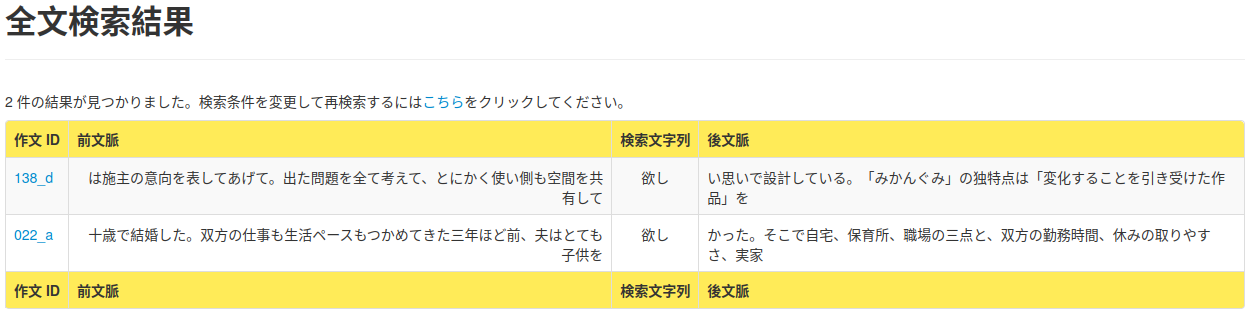
\includegraphics[width=\textwidth]{images/Exempel på resultat av sökning}
\end{figure}

\noindent
För att säkerställa att stavning med såväl \emph{kanji} som \emph{kana} ingick i sökresultatet, var det nödvändigt att genomföra dessa sökningar var för sig.

% Undersökningen
% Tillvägagångssätt
% Klassificering av data
\subsubsection{Klassificering av data}
\label{subsec:Undersökningen: Tillvägagångssätt: Klassificering av data}
I nästa steg klassificerades träffarna utifrån korrekt respektive felaktigt språkbruk. För varje sökträff noterades uppgift om författare, sökord, meningens korrekthet samt i vilken person den var skriven. I (\ref{ex:Natane1}) visas ett exempel på oacceptabel användning som hämtats ur korpusen. En tredje persons mentala tillstånd berördes och således borde den evidentiella markören \emph{garu} ha använts. På motsvarande sätt klassificerades i stället (\ref{ex:Natane2}) som acceptabel, då meningen var skriven i första person och inte krävde någon evidentiell markör. Ingen egen bedömning av meningarnas korrekthet gjordes, utan  denna baserades i sin helhet på den klassificering av språkfel som redan hade gjorts av modersmålstalare och ingick som en del i korpusen.

\begin{exe}
\ex[*]{
\label{ex:Natane1}
\gll Otto wa totemo kodomo o hoshi-katta. \\
     make \textsc{top} mycket barn \textsc{acc} vill-\textsc{pst} \\
\glt 'Min make ville väldigt gärna ha barn.'}
\end{exe}

\begin{exe}
\ex
\label{ex:Natane2}
\gll Sono kodomotachi o mi-te, ureshiku-naku-nari-masu. \\
     dessa barn \textsc{acc} se-\textsc{ger} glad-\textsc{neg}-bli-\textsc{pol}.\textsc{npst} \\
\glt 'Jag blir inte glad över att se de där barnen.'
\end{exe}

Då information om informanternas kunskapsnivå saknades, gjordes en uppskattning utifrån andra data som förekom i korpusen. Följande antagande gjordes: Talare med en hög kunskapsnivå skriver mer omfattande texter med längre meningar samtidigt som de gör färre språkfel jämfört med en mindre kunnig talare. Textens längd och meningarnas komplexitet ställdes i relation till de språkfel som förekom. Utifrån detta gjordes en matematisk beräkning där textens längd dividerades med det totala antalet förekommande språkfel. Detta skedde för samtliga informanter, vars texter förekom i korpusundersökningen. Därefter rangordnades dessa utifrån materialets uppskattade komplexitet. Rangordningen användes för att undersöka om det fanns några skillnader i språkbruk mellan de informanter som hade bedömts skriva mer respektive mindre komplexa texter.

% Undersökningen
% Tillvägagångssätt
% Statistisk testning
\subsubsection{Statistisk testning}
\label{subsec:Undersökningen: Tillvägagångssätt: Statistisk testning}
Avslutningsvis användes statistisk testning i form av hypotesprövning, för att försöka besvara de aktuella frågeställningarna. Först ställdes en nollhypotes upp, enligt vilken ingen statistiskt signifikant skillnad gick att påvisa. Därefter prövades korpusdata mot nollhypotesen med hjälp av statistiska tester. Då det funnits anledning att anta att urvalet inte skulle vara normalfördelat, behövde så kallade icke-parametriska metoder användas. Det var sannolikt ett lämpligt val, då de är tillämpbara på snedfördelat data. En konsekvens av det var dock att testets statistiska styrka samtidigt blev lägre \autocite{henriksson2008}.

En risk som inte helt kan uteslutas vid hypotesprövning är att nollhypotesen avfärdas trots att den är sann, vilket vanligtvis benämns typ I-fel. På motsvarande vis finns det en risk för att nollhypotesen felaktigt antas vara sann trots att den är falsk. Det kallas i stället för typ II-fel. Genom att göra genomtänkta val av statistiska tester kan dessa risker minimeras. \textcite[206]{körner2015} ger följande sammanfattning:

\blockquote{Lägg märke till att hypotesprövningen kan resultera i två typer av felaktiga beslut. \emph{Vi kan förkasta nollhypotesen när den är korrekt.} Detta felbeslut innebär att vi bedömer att materialet är användbart trots att det inte uppfyller de krav vi ställer. [...] \emph{Vi kan acceptera (inte förkasta) nollhypotesen när den är felaktig.} Det innebär att vi bedömer att materialet inte är användbart trots att det uppfyller de ställda kraven.}

\noindent
I huvudsak använde jag mig av chitvå-test i min undersökning, vilket kan vara ett lämpligt val för att mäta om det finns en statistiskt signifikant skillnad mellan förväntad och observerad frekvens, eller, annorlunda uttryckt, om två variabler är beroende av varandra eller ej. Korrekt användning av chitvå-test förutsätter dock att alla observationer är oberoende av varandra, vilket inte en korpusundersökning kan uppfylla fullt ut. Oavsett hur noggrant korpusens material har samlats in kan det inte till fullo motsvara ett helt slumpmässigt urval \autocite{brezina2018,körner2015}.




% Resultat %%%%%%%%%%%%%%%%%%%%%%%%%%%%%%%%%%%%%%%%%%%%%%%%%%%%%%%%%%%%%%%%%%%%%%%%%%%%%%%%%%%%%%%%%
%%%%%%%%%%%%%%%%%%%%%%%%%%%%%%%%%%%%%%%%%%%%%%%%%%%%%%%%%%%%%%%%%%%%%%%%%%%%%%%%%%%%%%%%%%%%%%%%%%%%
\newpage
\section{Resultat}
\label{ch:Resultat}
I resultatkapitlet presenteras den genomförda korpusundersökningen. Jag inleder kapitlet med en översiktlig genomgång av det material som har samlats in ur korpusen. Data om antal språkfel presenteras dels för urvalet i sin helhet, dels särredovisat utifrån kategori av mentalt verb. Språkbruk grupperat utifrån uppskattad komplexitet hos informanternas texter visas också. Därefter genomförs olika typer av statistiska tester, för att undersöka om det finns någon skillnad bland olika typer av texter. Sammanfattningsvis har det visat sig finnas en statistiskt signifikant skillnad mellan korrekt respektive felaktigt bruk av mentala verb bland de informanter, vars texter bedömts vara mindre komplexa. I denna grupp har också en positiv korrelation mellan korrekt respektive felaktigt språkbruk identifierats. Inga andra statistiskt säkerställda skillnader har kunnat beläggas.

% Resultat
% Utvärdering av korpusdata
\subsection{Utvärdering av korpusdata}
\label{sec:Resultat: Utvärdering av korpusdata}
Sammanlagt 462 förekomster av mentala verb bedömdes inom ramen för min korpusundersökning, vilka närmare framgår av tabell \ref{tab:Korpusdata1}. Nästan hälften av dessa kunde härledas till texter författade av modersmålstalare av marathi. Det bör ställas i proportion till det totala antalet informanter, där den gruppen utgjorde knappt en femtedel av dessa. Modersmålstalare av marathi var samtidigt den grupp som i såväl absoluta som relativa tal gjorde flest språkfel relaterade till bruket av mentala verb.

\begin{table}[h]
\caption{Resultat grupperat utifrån informanternas modersmål}
\label{tab:Korpusdata1}
\begin{tabular}{lSSSSSS}
\toprule
{} & \multicolumn{3}{c}{Språkbruk} & \multicolumn{3}{c}{Mentalt verb} \\
\cmidrule(rl){2-4} \cmidrule(rl){5-7}
Modersmål      & {Korrekt}    & {Felaktigt}  & {Summa}      & {Psykologiskt}    & {Fysiologiskt}    & {Summa} \\
\cmidrule(rl){1-1} \cmidrule(rl){2-3} \cmidrule(rl){4-4} \cmidrule(rl){5-6} \cmidrule(rl){7-7}
Marathi        & 177          & 41           & 218          & 218               & 0                 & 218 \\
Kinesiska      & 143          & 23           & 166          & 151               & 15                & 166 \\
Vietnamesiska  & 31           & 3            & 34           & 34                & 0                 & 34  \\
Koreanska      & 22           & 5            & 27           & 27                & 0                 & 27  \\
Slovenska      & 4            & 0            & 4            & 4                 & 0                 & 4   \\
Malajiska      & 2            & 0            & 2            & 2                 & 0                 & 2   \\
Spanska        & 1            & 1            & 2            & 2                 & 0                 & 2   \\
Uppgift saknas & 8            & 1            & 9            & 9                 & 0                 & 9   \\
\cmidrule(rl){1-7}
Summa          & 388          & 74           & 462          & 447               & 15                & 462 \\
\bottomrule
\end{tabular}
\end{table}

\noindent
Utöver den stora gruppen marathitalare så förekom också modersmålstalare av kinesiska, vietnamesiska och koreanska relativt frekvent. Däremot påträffades inte träffar från talare av malajiska, slovenska eller spanska i någon större utsträckning. Inget resultat kunde bedömas från modersmålstalare av ungerska eller thai. Dessa saknades helt i resultatet trots att de förekom i korpusen i övrigt. Redovisningen av dessa har därför också utelämnats i resultatkapitlet.

% Resultat
% Utvärdering av korpusdata
% Psykologiska mentala verb
\subsubsection{Psykologiska mentala verb}
\label{subsec:Resultat: Utvärdering av korpusdata: Psykologiska mentala verb}
Merparten av de mentala verb som förekom i korpusundersökningen härrörde sig till psykologiska fenomen i någon form. Samtliga mentala verb som \textcite{makino1986} kategoriserat som beskrivandes psykologiska fenomen förekom i någon utsträckning i resultatet, vilket framgår av tabell \ref{tab:Korpusdata2}. Fördelningen mellan dessa visade sig dock vara skev, där konstruktionen \emph{V$\sim$tai} ’vilja göra’ tillsammans med \emph{omoshiroi} ’vara intressant’ utgjorde en stor del av resultatet. Det bör samtidigt tydliggöras att konstruktionen \emph{V$\sim$tai} ’vilja göra’ kunde användas betydligt friare av informanterna jämfört med övriga mentala verb.\footnote{Genom att lägga till suffixet efter ett verbs \emph{reny\=okei}-form uttrycker talaren att denne vill utföra den handling som det aktuella verbet motsvarar. Eftersom spännvidden för en sådan konstruktion blir större än för ett specifikt mentalt verb, torde inte den höga frekvensen i sig vara särskilt anmärkningsvärd.}

\begin{table}[h]
\caption{Psykologiska mentala verb som förekom i korpusundersökningen}
\label{tab:Korpusdata2}
\begin{tabular}{llSSS}
\toprule
\multicolumn{2}{c}{} & \multicolumn{3}{c}{Språkbruk} \\
\cmidrule(rl){3-5}
\multicolumn{2}{c}{Mentalt verb}     & {Korrekt}    & {Felaktigt}  & {Summa} \\
\cmidrule(rl){1-2} \cmidrule(rl){3-4} \cmidrule(rl){5-5}
\emph{V$\sim$tai}   & 'vilja göra'           & 283          & 45           & 328 \\
\emph{omoshiroi}    & 'vara intressant'      & 49           & 8            & 57  \\
\emph{hoshii}       & 'vilja ha'             & 11           & 11           & 22  \\
\emph{ureshii}      & 'vara glad'            & 9            & 3            & 12  \\
\emph{kowai}        & 'vara rädd'            & 6            & 2            & 8   \\
\emph{sabishii}     & 'vara ensam'           & 8            & 0            & 8   \\
\emph{iyada}        & 'ogilla'               & 4            & 1            & 5   \\
\emph{meiwakuda}    & 'vara besvärlig'       & 2            & 2            & 4   \\
\emph{urayamashii}  & 'vara avundsjuk'       & 3            & 0            & 3   \\
\cmidrule(rl){1-5}
\multicolumn{2}{l}{Summa}                    & 375          & 72           & 447 \\
\bottomrule
\end{tabular}
\end{table}

\noindent
Mentala verb tillhörande ordklassen \emph{keiy\=od\=oshi} ’nominaladjektiv’ förekom endast nio gånger i resultatet, vilket motsvarar ungefär två procent av alla träffar. Det bör ställas i proportion till de 447 träffar som utgjorde samtliga förekomster av psykologiska mentala verb i korpusundersökningen. Totalt åtta informanter använde sig av dessa, varav sex var modersmålstalare av kinesiska. De resterande två förekomsterna var fördelade mellan talare av koreanska och vietnamesiska.

% Resultat
% Utvärdering av korpusdata
% Fysiologiska mentala verb
\subsubsection{Fysiologiska mentala verb}
\label{subsec:Resultat: Utvärdering av korpusdata: Fysiologiska mentala verb}
Frekvensen av mentala verb som behandlade fysiologiska fenomen visade sig vara lägre än för motsvarande psykologiska företeelser. Av tabell \ref{tab:Korpusdata1} ovan framgår att de enda förekomsterna fanns bland modersmålstalare av kinesiska; frekvensen var dock låg också bland dessa talare. Enbart tio informanter använde sig över huvud taget av något fysiologiskt mentalt verb, vilket bör ställas i proportion till de sammanlagt 115 stycken talare av kinesiska som förekom i korpusen.

\begin{table}[h]
\caption{Fysiologiska mentala verb som förekom i korpusundersökningen}
\label{tab:Korpusdata3}
\begin{tabular}{llSSS}
\toprule
\multicolumn{2}{c}{} & \multicolumn{3}{c}{Språkbruk} \\
\cmidrule(rl){3-5}
\multicolumn{2}{c}{Mentalt verb}     & {Korrekt}    & {Felaktigt}  & {Summa} \\
\cmidrule(rl){1-2} \cmidrule(rl){3-4} \cmidrule(rl){5-5}
\emph{itai}         &    'göra ont'          & 5            & 0            & 5  \\
\emph{samui}        &    'vara kall'         & 5            & 0            & 5  \\
\emph{kurushii}     &    'göra ont'          & 1            & 2            & 3  \\
\emph{darui}        &    'vara orkeslös'     & 2            & 0            & 2  \\
\cmidrule(rl){1-5}
\multicolumn{2}{l}{Summa}                    & 13           & 2            & 15 \\
\bottomrule
\end{tabular}
\end{table}

\noindent
Av tabell \ref{tab:Korpusdata3} framgår att tre av de sju fysiologiska mentala verb som räknades av upp \textcite{makino1986} helt saknades i korpusundersökningens resultat. Det visades sig att varken \emph{kayui} 'klia', \emph{atsui} 'vara varm' eller \emph{kusuguttai} 'vara kittlig' förekom i någon form.\footnote{Jag var noga med att kontrollera resultatet, då \emph{atsui} 'vara varm' kan skrivas med olika \emph{kanji} beroende på om det är ett varmt föremål eller en varm person som avses. Det mentala verbet torde enbart avse en persons fysiologiska tillstånd. Trots det fanns det inga relevanta träffar i korpusen.} Det enda felaktiga bruket hittades bland \emph{kurushii} 'göra ont', där två informanter gjorde ett språkfel vardera. En av informanterna använde mentala verb korrekt i två andra fall, medan den andre inte använde dem korrekt någon gång.

% Resultat
% Hypotesprövning
\subsection{Hypotesprövning}
\label{sec:Resultat: Hypotesprövning}
Chitvå-test användes för att undersöka förhållandet mellan korrekt respektive felaktigt språkbruk i första respektive tredje person. Först genomfördes ett test av urvalet i sin helhet och därefter var för sig för de informanter, vars texter hade bedömts vara mer respektive mindre komplexa än medianen. Slutligen beräknades Pearsons korrelationskoefficient för att bestämma om det fanns någon statistiskt signifikant korrelation mellan frekvensen av korrekt respektive felaktigt språkbruk. Konfidensgraden 95 procent användes genomgående för de genomförda statistiska testerna.

% Resultat
% Hypotesprövning
% Hypotesprövning av hela urvalet
\subsubsection{Hypotesprövning av hela urvalet}
\label{subsec:Resultat: Hypotesprövning: Hypotesprövning av hela urvalet}
Hur fördelningen av korrekt respektive felaktigt språkbruk såg ut i första respektive tredje person för urvalet i sin helhet framgår av tabell \ref{tab:Chitvå1}. Det fanns inget statistiskt signifikant samband mellan dessa variabler, $\chi$^{2}(2, \emph{N} = 117) = 0,73, \emph{p} = 0,392. Nollhypotesen, det finns inte någon skillnad mellan korrekt respektive felaktigt språkbruk i första respektive tredje person, kunde således inte förkastas.

\begin{table}[h]
\caption{Utvärdering av språkbruk för urvalet i sin helhet}
\label{tab:Chitvå1}
\begin{tabular}{lSSS}
\toprule
{} & \multicolumn{3}{c}{Språkbruk} \\
\cmidrule(rl){2-4}
{}   & {Korrekt}    & {Felaktigt}  & {Summa} \\
\cmidrule(rl){2-3} \cmidrule(rl){4-4}
{Första person}     & 296     & 53      & 349 \\
{Tredje person}     & 92      & 21      & 113 \\
\cmidrule(rl){1-4}
Summa               & 388     & 74      & 462 \\
\bottomrule
\end{tabular}
\end{table}

\noindent
Ingen statistiskt signifikant korrelation mellan frekvensen av korrekt respektive felaktigt språkbruk kunde påvisas, \emph{r}(115) = 0,07, \emph{p} = 0,476.

% Resultat
% Hypotesprövning
% Hypotesprövning för texter med högre grad av komplexitet
\subsubsection{Hypotesprövning för texter med högre grad av komplexitet}
\label{subsec:Resultat: Hypotesprövning: Hypotesprövning för texter med högre grad av komplexitet}
Av tabell \ref{tab:Chitvå2} framgår hur fördelningen av korrekt respektive felaktigt språkbruk såg ut i den övre halvan av urvalet, det vill säga bland de informanter, vars texter som enligt min skattningsmodell hade bedömts vara mer komplexa än medianen. För den övre halvan av urvalet fanns det inget statistiskt signifikant samband mellan korrekt respektive felaktigt språkbruk i första respektive tredje person, $\chi$^{2}(2, \emph{N} = 59) = 0,71, \emph{p} = 0,340, och därmed kunde inte nollhypotesen förkastas.

\begin{table}[h]
\caption{Utvärdering av språkbruk för texter med högre grad av komplexitet}
\label{tab:Chitvå2}
\begin{tabular}{lSSS}
\toprule
{} & \multicolumn{3}{c}{Språkbruk} \\
\cmidrule(rl){2-4}
{}   & {Korrekt}    & {Felaktigt}  & {Summa} \\
\cmidrule(rl){2-3} \cmidrule(rl){4-4}
{Första person}     & 155     & 20      & 175 \\
{Tredje person}     & 60      & 5       & 65  \\
\cmidrule(rl){1-4}
Summa               & 215     & 25      & 240 \\
\bottomrule
\end{tabular}
\end{table}

\noindent
Det fanns en svagt negativ korrelation mellan frekvensen av korrekt respektive felaktigt språkbruk, \emph{r}(57) = -0,24, \emph{p} = 0,064; resultatet var dock inte statistiskt signifikant. En statistiskt säkerställd negativ korrelation skulle ha inneburit att ju oftare en talare använder mentala verb korrekt, desto mer sällan använder denne dem också felaktigt.

% Resultat
% Hypotesprövning
% Hypotesprövning för texter med lägre grad av komplexitet
\subsubsection{Hypotesprövning för texter med lägre grad av komplexitet}
\label{subsec:Resultat: Hypotesprövning: Hypotesprövning för texter med lägre grad av komplexitet}
Av tabell \ref{tab:Chitvå3} framgår hur fördelningen av korrekt respektive felaktigt språkbruk såg ut i den undre halvan av urvalet, det vill säga bland de informanter, vars texter som enligt min skattningsmodell hade bedömts vara mindre komplexa än medianen. För den under halvan av urvalet fanns det ett statistiskt signifikant samband mellan korrekt respektive felaktigt språkbruk i första respektive tredje person, $\chi$^{2}(2, \emph{N} = 58) = 4,52, \emph{p} = 0,034, och nollhypotesen förkastades således. Det felaktiga språkbruket i tredje person var mer frekvent än vad som hade kunnat förväntas av en jämn fördelning.

\begin{table}[h]
\caption{Utvärdering av språkbruk för texter med lägre grad av komplexitet}
\label{tab:Chitvå3}
\begin{tabular}{lSSS}
\toprule
{} & \multicolumn{3}{c}{Språkbruk} \\
\cmidrule(rl){2-4}
{}   & {Korrekt}    & {Felaktigt}  & {Summa} \\
\cmidrule(rl){2-3} \cmidrule(rl){4-4}
{Första person}     & 141     & 33      & 174 \\
{Tredje person}     & 32      & 16      & 48  \\
\cmidrule(rl){1-4}
Summa               & 173     & 49      & 222 \\
\bottomrule
\end{tabular}
\end{table}

\noindent
Det fanns en svagt positiv korrelation mellan frekvensen av korrekt respektive felaktigt språkbruk, \emph{r}(56) = 0,32, \emph{p} = 0,015; resultatet var statistiskt signifikant. En positiv korrelation mellan variablerna korrekt respektive felaktigt språkbruk innebär att ju oftare en talare använder mentala verb korrekt, desto oftare kommer denne också att använda dem felaktigt. Det kan vid en första anblick möjligen upplevas som motsägelsefull, men kommer att utvecklas närmare i det efterföljande diskussionskapitlet.

Sammanfattningsvis utvärderades 462 stycken förekomster av mentala verb inom ramen för korpusundersökningen. Av dessa bedömdes 388 stycken användas korrekt och 74 stycken felaktigt. Merparten av de mentala verb som ingick i resultatet beskrev olika typer av psykologiska fenomen. Enbart ett mindre antal fysiologiska mentala verb förekom. Det har visat sig finnas en statistiskt signifikant skillnad mellan korrekt respektive felaktigt bruk av mentala verb bland de informanter, vars texter bedömts vara mindre komplexa. I denna grupp har också en positiv korrelation mellan korrekt respektive felaktigt språkbruk identifierats. Inga andra statistiskt säkerställda skillnader har kunnat beläggas.




% Diskussion %%%%%%%%%%%%%%%%%%%%%%%%%%%%%%%%%%%%%%%%%%%%%%%%%%%%%%%%%%%%%%%%%%%%%%%%%%%%%%%%%%%%%%%
%%%%%%%%%%%%%%%%%%%%%%%%%%%%%%%%%%%%%%%%%%%%%%%%%%%%%%%%%%%%%%%%%%%%%%%%%%%%%%%%%%%%%%%%%%%%%%%%%%%%
\newpage
\section{Diskussion}
\label{ch:Diskussion}

% Diskussion
% Resultatdiskussion
\subsection{Resultatdiskussion}
\label{sec:Diskussion: Resultatdiskussion}
Modersmålstalare av marathi, ett indoeuropeiskt språk som talas i västra Indien, utgjorde ungefär en femtedel av korpusens totala sammansättning av informanter. Trots det stod den gruppen för nästan hälften av all användning av mentala verb i undersökningen. Den största delen av dessa härrörde sig till meningar som inte var särskilt komplexa. Texterna handlade nästan alltid om önskningar och förhoppningar om framtiden och hade en förhållandevis okomplicerad satsstruktur. I skarp kontrast till det stod texter skrivna av främst kinesiska och koreanska inlärare. Dessa var generellt sett de mest komplexa ur såväl ett innehållsmässigt som syntaktiskt perspektiv. Här berördes till exempel ämnen som livstids fängelse och dödsstraff, politiska åsikter samt självmord.

Det skeva förhållandet mellan frekvensen av psykologiska respektive fysiologiska mentala verb i undersökningen är svårförklarat. Jag har inte kunnat hitta några belägg i litteraturen för att den ena typen skulle vara vanligare än den andra. Inte heller har det funnits någon sådan notering i anslutning till den lista över mentala verb som användes för att välja ut sökord. Frekvensen för respektive mentalt verb skulle behöva analyseras närmare, för att bättre kunna avgöra om resultatet avviker från vad som hade kunnat förväntas.

Inga exempel på användning av mentala verb i andra person förekom i resultatet. Det torde till viss del kunna förklaras utifrån användningen av en inlärarkorpus där enbart skriven text ingick. Då användningen av mentala verb i andra person begränsas till frågesatser, verkar det sannolikt att de tillfällen när dessa skulle kunna förekomma naturligt i skriven text är få. Resultatet hade möjligen blivit ett annat om i stället en inlärarkorpus med transkriberat tal hade använts. En direkt konsekvens av det var att generaliserbarheten för undersökningen minskade. Det vore således lämpligare att utifrån studiens resultat främst diskutera de språkfel som hänförde sig till en skriven kontext.

Det språkfel som förekom mest frekvent i min undersökning torde vara hyperkorrektioner av olika slag. Dessa tog sig ofta uttryck i att informanten använde en evidentiell markör när en sådan inte krävdes. I såväl (\ref{ex:Natane3}) som (\ref{ex:Natane4}) har den sortens språkfel kunnat identifieras. Användningen av en evidentiell markör är en syntaktiskt mer komplex konstruktion än att i stället utelämna den, vilket talar emot att den skulle ha använts av misstag. I stället verkar det ha skett ett aktivt val i en strävan att uttrycka sig på ett uppfattat korrekt sätt.

\begin{exe}
\ex[*]{
\label{ex:Natane3}
\gll Watashi wa anata no sensei ni nat-te mi-te hoshi-gat-te desu. \\
     jag \textsc{top} du \textsc{gen} lärare \textsc{dat} bli-\textsc{ger} försöka-\textsc{ger} vill-\textsc{evid}-\textsc{ger} \textsc{cop}.\textsc{pol}.\textsc{npst} \\
\glt 'Jag vill att du ska bli min lärare.'}
\end{exe}

\begin{exe}
\ex[*]{
\label{ex:Natane4}
\gll Ureshii toki mo ureshii-dewanai toki mo ongaku o kiki-ta-gat-te-i-masu. \\
     glad tid \textsc{foc} glad-\textsc{cop}.\textsc{neg} tid \textsc{foc} musik \textsc{acc} lyssna-vill-\textsc{evid}-\textsc{ger}-vara-\textsc{pol}.\textsc{npst} \\
\glt 'Jag tycker om att lyssna på musik både när jag är glad och när jag är ledsen.'}
\end{exe}

Det är inte alltid särskilt enkelt, eller ens meningsfullt, att skilja språkfel av kategorierna hyperkorrektion respektive övergeneralisering från varandra. I det här fallet, när möjligheten att fråga informanten om hur denne resonerade saknas, blir det i någon mån en subjektiv bedömning baserad på vad som verkar mest sannolikt utifrån den givna kontexten. Ett sådant fall har kunnat identifieras i (\ref{ex:Natane5}). Meningen innefattade, utöver det felaktiga valet av konjunktion, en ogrammatisk användning av \emph{naritai} 'vilja bli' i anslutning till en bisats, vilket var intressant ur det perspektivet.

\begin{exe}
\ex[*]{
\label{ex:Natane5}
\gll Ry\=oshin wa watashi ni gink\=oin ni nari-ta-gat-te kara, iroiro na gink\=o no shiken mo uke-mashita. \\
     föräldrar \textsc{top} jag \textsc{dat} bankman \textsc{dat} bli-vill-\textsc{evid}-\textsc{ger} eftersom olika \textsc{cop} bank \textsc{gen} prov \textsc{foc} ta-\textsc{pol}.\textsc{pst} \\
\glt 'Jag skrev olika sorters prov eftersom mina föräldrar vill att jag ska bli bankman.'}
\end{exe}

\noindent
Ett mentalt tillstånd hos informantens föräldrar och inte denne själv beskrevs, vilket sannolikt talade för användningen av en evidentiell markör. I det här fallet var det dock felaktigt, då grammatisk användning av mentala verb i anslutning till bisatser kräver att de uttrycks utan någon evidentiell markör. Informanten verkar inte ha behärskat den grammatiska regeln fullt ut. Den har i stället använts alltför generellt, vilket stämmer väl överens med den beskrivning av övergeneralisering som finns i litteraturen.

Transfer, oönskad påverkan från ett annat språk, har inte kunnat identifieras i någon större utsträckning. Det i sig torde inte vara särskilt förvånande, då jag inte är modersmålstalare av något av de språk som utgjorde informanternas modersmål. Trots det fanns det vissa träffar som bedömdes ha kunnat hänföra sig till denna typ av språkfel. På exempelvis svenska och engelska uttrycks talarens vilja i form av ett verb, att vilja, medan motsvarande yttrande rent syntaktiskt tillhör ordklassen \emph{keiy\=oshi} 'äkta adjektiv' på japanska. I undersökningen har det visat sig finnas vissa belägg för denna problematik.

\begin{exe}
\ex[*]{
\label{ex:Natane6}
\gll Watashi wa okane yori jibun no ii koto nitsuite y\=umei ni naru {to iu} koto ga hoshii desu. \\
     jag \textsc{top} pengar mindre egen \textsc{gen} bra sak rörande känd \textsc{dat} bli \textsc{comp} sak \textsc{nom} vill \textsc{cop}.\textsc{pol}.\textsc{npst} \\
\glt 'Jag vill hellre bli berömd för mina goda gärningar än för min förmögenhet.'}
\end{exe}

\begin{exe}
\ex[*]{
\label{ex:Natane7}
\gll Watashi wa nihongo o tsukau shigoto o shi-te hoshii desu. \\
     jag \textsc{top} japanska \textsc{acc} använda arbete \textsc{acc} göra-\textsc{ger} vill \textsc{cop}.\textsc{pol}.\textsc{npst} \\
\glt 'Jag vill ha ett arbete där jag kan använda min japanska.'}
\end{exe}

\noindent
I såväl (\ref{ex:Natane6}) som (\ref{ex:Natane7}) gav informanterna uttryck för sina egna önskemål. Det var i huvudsak den felaktiga användningen av det mentala verbet \emph{hoshii} 'vilja ha' i stället för konstruktionen \emph{V$\sim$tai} 'vilja göra' som gjorde meningarna ogrammatiska. På japanska är den typen av konstruktion som informanterna har använt sig av reserverad för det fall när talaren uttrycker en önskan om vad en annan person ska göra. I den aktuella kontexten hade i stället det lämpliga valet varit just konstruktionen \emph{V$\sim$tai} 'vilja göra'.

Jag har tidigare gjort ett antagande om att de mer komplexa texterna skulle vara skrivna av talare med en högre kunskapsnivå och omvänt. Givet att det antagandet var korrekt så verkar resultaten från de genomförda statistiska testerna stämma förhållandevis väl med vad som kan antas vara intuitivt riktigt. Bland den grupp informanter som hade bedömts skriva mer komplexa texter fanns det inga belägg för att bruket av mentala verb skulle vara mer komplicerat i tredje person. Det fanns också en svagt negativ korrelation mellan korrekt respektive felaktigt språkbruk, vilket innebär att en talare som använde mentala verb korrekt också var mindre benägen att använda dem felaktigt. En möjlig tolkning av dessa resultat är att det fanns en medvetenhet om restriktionerna på mentala verb. Motsvarande iakttagelse har inte kunnat göras bland den andra gruppen informanter.

Bland de informanter som hade bedömts skriva mindre komplexa texter fanns de enda resultat i undersökningen som var statistiskt signifikanta. Frekvensen av språkfel i tredje person var högre än vad som hade kunnat förväntas. Det innebär att det var vanligare att göra språkfel i tredje person jämfört med i första person. Vidare fanns det i den här gruppen en positiv korrelation mellan korrekt respektive felaktigt språkbruk. Jag menar att det skulle kunna förstås som att det inte fanns någon medvetenhet om restriktionerna på mentala verb. I stället för att göra ett medvetet val ledde slumpen till att resultatet ibland blev korrekt och ibland felaktigt. Sammantaget skulle det kunna tyda på att restriktionerna på mentala verb inte behärskades fullt ut i denna grupp.

% Diskussion
% Metoddiskussion
\subsection{Metoddiskussion}
\label{sec:Diskussion: Metoddiskussion}
En av korpuslingvistikens grundprinciper torde vara att en korpus ska fungera som ett stickprov ur en större population; en inlärarkorpus representerar exempelvis de personer som lär sig ett främmande språk. Det kan vara en välfungerande metod för att se mönster i exempelvis språkanvändningen hos denna grupp. På samma gång krävs det en medvetenhet om att det inte är möjligt att avgöra hur väl korpusen faktiskt representerar en specifik population, vilket kan få negativ påverkan på resultatets generaliserbarhet.

Närmare 60 procent av de informanter som valdes ut utgjordes av modersmålstalare av kinesiska. Därefter följde talare av olika typer av indoeuropeiska språk, vilka tillsammans omfattade ungefär 20 procent av andelen informanter. Andra typer av språkfamiljer fanns också representerade, där exempelvis austroasiatiska respektive koreanska språk förekom i några fall. Då det var informanternas förståelse för ett potentiellt främmande kulturellt förhållningssätt som avsågs att studeras, torde också den kulturella bakgrunden ha varit av vikt för resultatet. Möjligen skulle detta kunna vara en faktor som påverkade generaliserbarheten negativt, då motsvarande undersökning med en annan sammansättning av informanter inte nödvändigtvis skulle ha gett samma resultat. För att säkerställa såväl hög validitet som reliabilitet, skulle undersökningen kunna upprepas med informanter med en annan kulturell bakgrund.

Ett annat möjligt problem kopplat till undersökningens validitet var korpusens sammansättning. Komplexiteten hos de ingående texterna hade en stor spännvidd, där delar av innehållet var på en grundläggande nivå. Som exempel kan nämnas att en stor del av materialet författat av marathitalare torde ha hört till nybörjarnivån. Dessa texter var, som jag har nämnt ovan, sällan särskilt komplexa i sin struktur. Det kan finnas både för- och nackdelar med det, då en inlärare i början av sina språkstudier torde ha haft mindre kännedom om de restriktioner på språkbruk som följer av kulturella skäl. I det här fallet visade sig texterna dock endast undantagsvis beröra en tredje persons känslor och önskningar. Enbart två exempel på sådan språkanvändning har kunnat identifieras i materialet. Det är olyckligt samtidigt som det belyser den metodologiska utmaningen med att inte på förhand kunna känna till vilken språklig nivå varje enskild text har.

Det har också funnits en viss problematik relaterad till den klassificering av språkfel som ingick i korpusen. I (\ref{ex:Natane8}) har meningen klassificerats som ogrammatisk, då den saknade en ackusativmarkör efter \emph{kanji}, vilket torde ha varit en korrekt bedömning. Problemet var att den föreslagna rättelsen samtidigt visade sig introducera ett nytt språkfel, då den utöver att påpeka det syntaktiska felet också föreslog att skrivtecknen för ordet \emph{kanji} borde bytas ut. Det skulle ha gett meningen en innebörd som inte passade in i den givna kontexten och bör rimligtvis ha varit ett misstag.

\begin{exe}
\ex[*]{
\label{ex:Natane8}
\gll Watashi wa minna ni kanji sh\=okai shi-tai to omoi-masu. \\
     jag \textsc{top} alla \textsc{dat} \emph{kanji} presentera göra-vill \textsc{quot} tänka-\textsc{pol}.\textsc{npst} \\
\glt 'Jag skulle vilja presentera kanji för er allihop.'}
\end{exe}

\noindent
Jag har inte kunnat identifiera några fler fel av den här typen, men menar att det fortfarande behöver beröras, i synnerhet då en betydande del av min undersökning har sin grund i denna klassificering av språkfel. Om den här sortens misstag hade varit mer frekvent förekommande, skulle det ha kunnat påverka undersökningens reliabilitet negativt.

Avslutningsvis bör det nämnas att inte alla antaganden som de genomförda statistiska testerna vilar på kunde uppfyllas fullt ut. En korrekt användning av chitvå-test förutsätter exempelvis att varje observation som görs är oberoende av resterande delar av urvalet. När data hämtas ur en korpus blir en naturlig följd av det att texterna i någon mån är relaterade till varandra, vilket medför att förutsättningen inte helt kan uppfyllas. Det här är ett övervägande som behöver göras inom ramen för varje korpusundersökning, men samtidigt krävs det en medvetenhet om att risken för typ I-fel, att felaktigt förkasta nollhypotesen trots att den är korrekt, därav ökar.

% Diskussion
% Framtida forskning
\subsection{Framtida forskning}
\label{sec:Diskussion: Framtida forskning}
Under tiden för uppsatsens skrivande har en fråga återkommit vid flera tillfällen: Hur kan de restriktioner som finns på mentala verb bäst förstås utifrån Kamios teori om informationsterritorium? Det har tidigare nämnts att det finns mentala verb som tvärtemot saknar de restriktioner som annars finns på deras användning. Vad kan vara anledningen till att det sker? På motsvarande vis uppträder en del statiska verb likt \emph{omou} 'att tänka' på i princip samma sätt som mentala verb. Det verkar inte osannolikt att skulle kunna ha med talarens tillgång till information att göra. Finns det fler statiska verb som beter sig på liknande vis? Vad kan i så fall vara anledningen till det? Det här torde kunna vara exempel på frågor värda att undersöka betydligt mer grundligt än vad som har varit möjligt att göra inom ramen för denna uppsats.




% Slutsatser %%%%%%%%%%%%%%%%%%%%%%%%%%%%%%%%%%%%%%%%%%%%%%%%%%%%%%%%%%%%%%%%%%%%%%%%%%%%%%%%%%%%%%%
%%%%%%%%%%%%%%%%%%%%%%%%%%%%%%%%%%%%%%%%%%%%%%%%%%%%%%%%%%%%%%%%%%%%%%%%%%%%%%%%%%%%%%%%%%%%%%%%%%%%
\newpage
\section{Slutsatser}
\label{ch:Slutsatser}
Den här uppsatsens syfte har dels varit att klarlägga hur bruket av mentala verb ser ut bland L2-talare av japanska, dels att belysa vilka språkfel som görs av dessa talare. Jag har genomfört en korpusundersökning och gjort sökningar i en inlärarkorpus, där eventuella språkfel redan i förväg hade identifierats av modersmålstalare av japanska. Totalt 16 stycken mentala verb, beskrivandes såväl psykologiska som fysiologiska fenomen, har fungerat som sökord i korpusen. Följande frågeställningar har försökts att besvaras:

\begin{itemize}
\item Vilka språkfel förekommer bland L2-talare av japanska?
\item I vilken mån tar L2-talare av japanska hänsyn till de restriktioner som finns på bruket av mentala verb?
\end{itemize}

Rörande den första frågeställningen så har jag funnit belägg för tre olika typer av språkfel. Det vanligaste av dessa har varit olika former av hyperkorrektioner, där talaren, i en strävan att uttrycka sig på ett uppfattat korrekt sätt, har använt mentala verb ogrammatiskt. Vidare har också exempel på övergeneralisering, att en grammatisk regel tillämpas alltför generellt, kunnat identifieras i materialet. Avslutningsvis har det funnits ett fåtal tillfällen där transfer, oönskad påverkan från ett annat språk, har kunnat vara en möjlig felorsak.

Beträffande den andra frågeställningen så har jag genomfört statistiska tester för att undersöka om frekvensen av språkfel har varit högre än vad som hade kunnat förväntas. Varken i urvalet i sin helhet eller bland den grupp informanter som har bedömts skriva mer komplexa texter har det funnits några belägg för det. Däremot har det funnits statistiskt signifikanta resultat bland den grupp informanter som har bedömts skriva mindre komplexa texter. I denna grupp har det kunnat beläggas att andelen språkfel i tredje person var högre än förväntat. En tänkbar förklaring skulle kunna vara att dessa informanter inte har tagit hänsyn till de restriktioner som finns på mentala verb fullt ut.




% Litteratur %%%%%%%%%%%%%%%%%%%%%%%%%%%%%%%%%%%%%%%%%%%%%%%%%%%%%%%%%%%%%%%%%%%%%%%%%%%%%%%%%%%%%%%
%%%%%%%%%%%%%%%%%%%%%%%%%%%%%%%%%%%%%%%%%%%%%%%%%%%%%%%%%%%%%%%%%%%%%%%%%%%%%%%%%%%%%%%%%%%%%%%%%%%%
\newpage
\printbibliography[heading=bibintoc,title=Litteratur]

\end{document}
